\documentclass[preview]{standalone}
\usepackage{tikz}
\usetikzlibrary{arrows}

\begin{document}
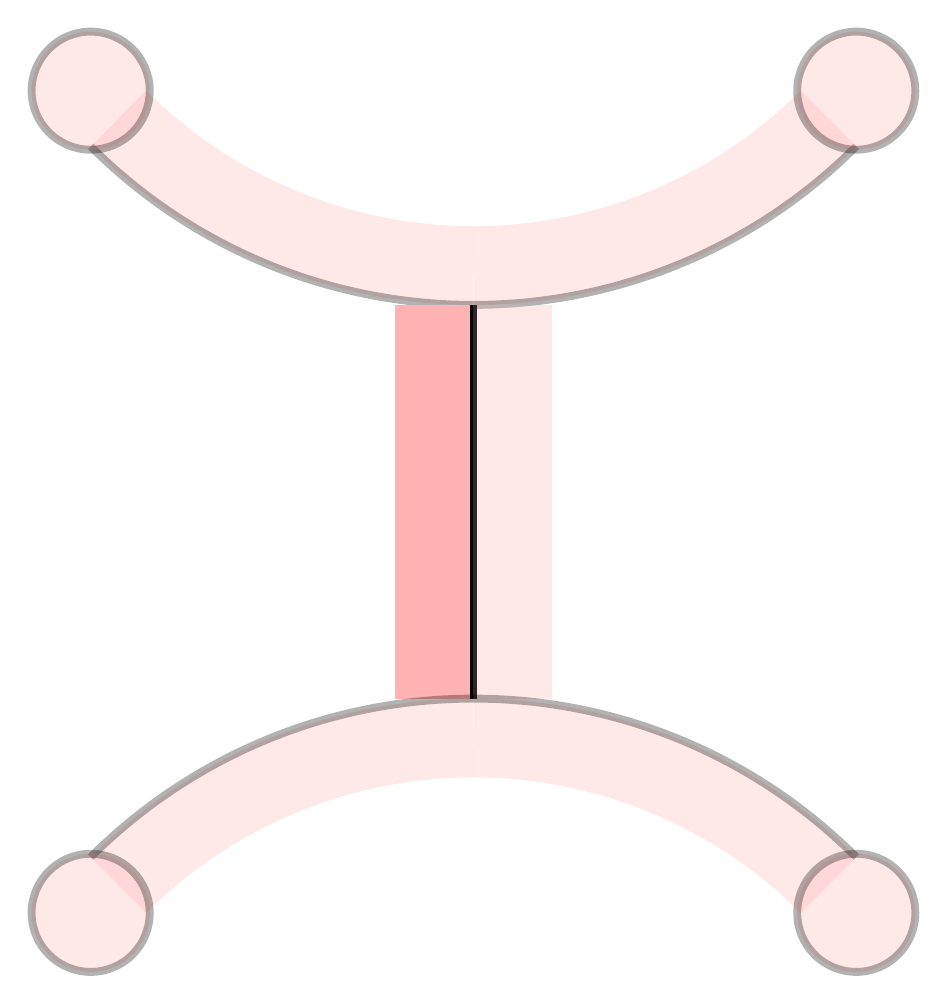
\begin{tikzpicture}[scale=1, 
stretch/.style={color=red!30, line width=1cm},
foot/.style={fill=red!30, line width=1mm},
solid/.style={line width=1mm}]

\def\legO{.3}
\def\legi{.3}
\def\legii{.3}
\def\legiii{.3}
\def\bellyiv{1}
\def\bellyv{.3}
\def\footvi{.3}
\def\footvii{.3}
\def\footviii{.3}
\def\footix{.3}



\def\pressure{50}
\def\hx{6}	
\def\hy{1}  % change only with line width of stretch
\def\lb{5}	% length of belly

\pgfmathsetmacro{\hyh}{.5*\hy}
\pgfmathsetmacro{\hxh}{\hx/2}

\pgfmathsetmacro{\alp}{90*\pressure/100}
\def\pi{3.1416}
\pgfmathsetmacro{\r}{\hx/\alp*180/\pi*.9}



% Bended
\begin{scope}[opacity = \legO]	% Leg 0
\draw[stretch] (0,0)arc(270:270-\alp:\r-\hyh)++(90+\alp:.5) coordinate(X);
\draw[solid] (0,-\hyh)arc(270:270-\alp:\r);
\end{scope}

\begin{scope}[opacity = \footvi]	% Foot 6
\draw[foot] (X) circle (.75);
\end{scope}

\begin{scope}[opacity = \legi]	% Leg 1
\draw[stretch] (0,0)arc(270:270+\alp:\r-\hyh) ++(\alp:.5)coordinate(X);
\draw[solid] (0,-\hyh)arc(270:270+\alp:\r);
\end{scope}


\begin{scope}[opacity = \footvii]	% Foot 7
\draw[foot] (X) circle (.75);
\end{scope}


\begin{scope}[opacity = \bellyiv]	% Belly 4
\draw[stretch] (-\hyh,-\hyh) --++ (0,-\lb);
\draw[solid] (0,-\hyh)--++(0,-\lb);
\end{scope}

\begin{scope}[opacity = \bellyv]	% Belly 5
\draw[stretch] (\hyh,-\hyh) --++ (0,-\lb);
\draw[solid] (0,-\hyh)--++(0,-\lb);
\end{scope}


\begin{scope}[opacity = \legii]	% Leg 2
\draw[stretch] (0,-\lb-\hy)arc(90:90+\alp:\r-\hyh)++(180+\alp:.5) coordinate(X);
\draw[solid] (0,-\lb-\hyh)arc(90:90+\alp:\r);
\end{scope}

\begin{scope}[opacity = \footviii]	% Foot 8
\draw[foot] (X) circle (.75);
\end{scope}


\begin{scope}[opacity = \legiii]	% Leg 3
\draw[stretch] (0,-\lb-\hy)arc(90:90-\alp:\r-\hyh)++(-\alp:.5) coordinate(X);
\draw[solid] (0,-\lb-\hyh)arc(90:90-\alp:\r);
\end{scope}

\begin{scope}[opacity = \footix]	% Foot 9
\draw[foot] (X) circle (.75);
\end{scope}

\end{tikzpicture}
\end{document}